\begin{figure}[h]
    \centering
    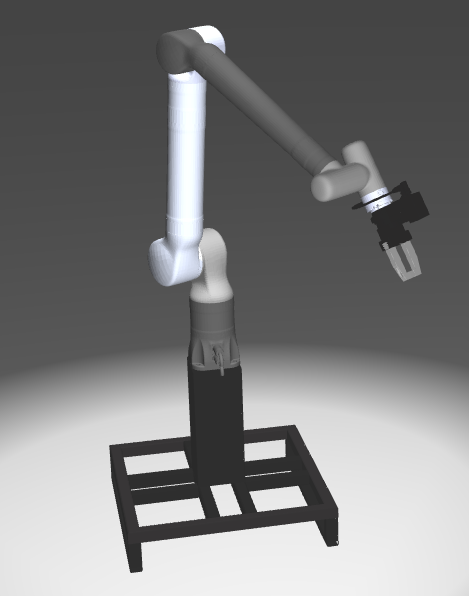
\includegraphics[width=0.3\textwidth]{figures/handling-robot-simulation.png}
    \caption{Handling Robot KR1410 in simulation}
    \label{fig:handling-robot-simulation}
\end{figure}
Handling robot is the primary robot which handles the sheet metal parts to different subsystems \textit{i.e.}
unloading station, bending machine and storage station.
It coordinates with the PLC to make decisions during the execution of the program. Reachability
is very important in this case, as it should be able to handle sheet metal parts in any orientation.
A two finger gripper is used for grasping the sheet metal parts.

To get accuracy with the bending process, detection of features on the sheet metal parts is required.
A robotic camera is mounted of the robot for this purpose. In this way, handling robot can be trained 
to operate with different variants of sheet metal parts.

ROS simulations of the handling robot is done to determine the performance of robot in the workcell.
The drawers of storage system is especially close
to the production floor and the robot requires some space to move around without getting stuck. 
Reachability is tested with the simulation of trajectories before the final integration of the real robot
in the workcell.